\section{Interpolation}
\subsection{Lagrange interpolation}
The \textit{unique} degree $n-1$ polynomial that interpolates the $n$ datapoints $(x_1, y_1), ..., (x_n, y_n)$ is given by
$$
P_{n-1}(x) = y_1L_1(x) + ... + y_nL_n(x)
$$
where $L_k$ is given by
\begin{gather*}
L_k(x) = \frac{(x-x_1)...(x-x_{k-1})(x-x_{k+1})...(x-x_n)}{(x_k-x_1)...(x_k - x_{k-1})(x_k - x_{k+1})...(x_k-x_n)}
\end{gather*}

\subsection{Netwon's divided differences}
\begin{definition}
Denote by $f[x_1...x_n]$ the coefficient of the $x^{n-1}$ term in the (unique) polynomial that interpolates $(x_1, f(x_1)), ..., (x_n,f(x_n))$.
\end{definition}

\begin{center}
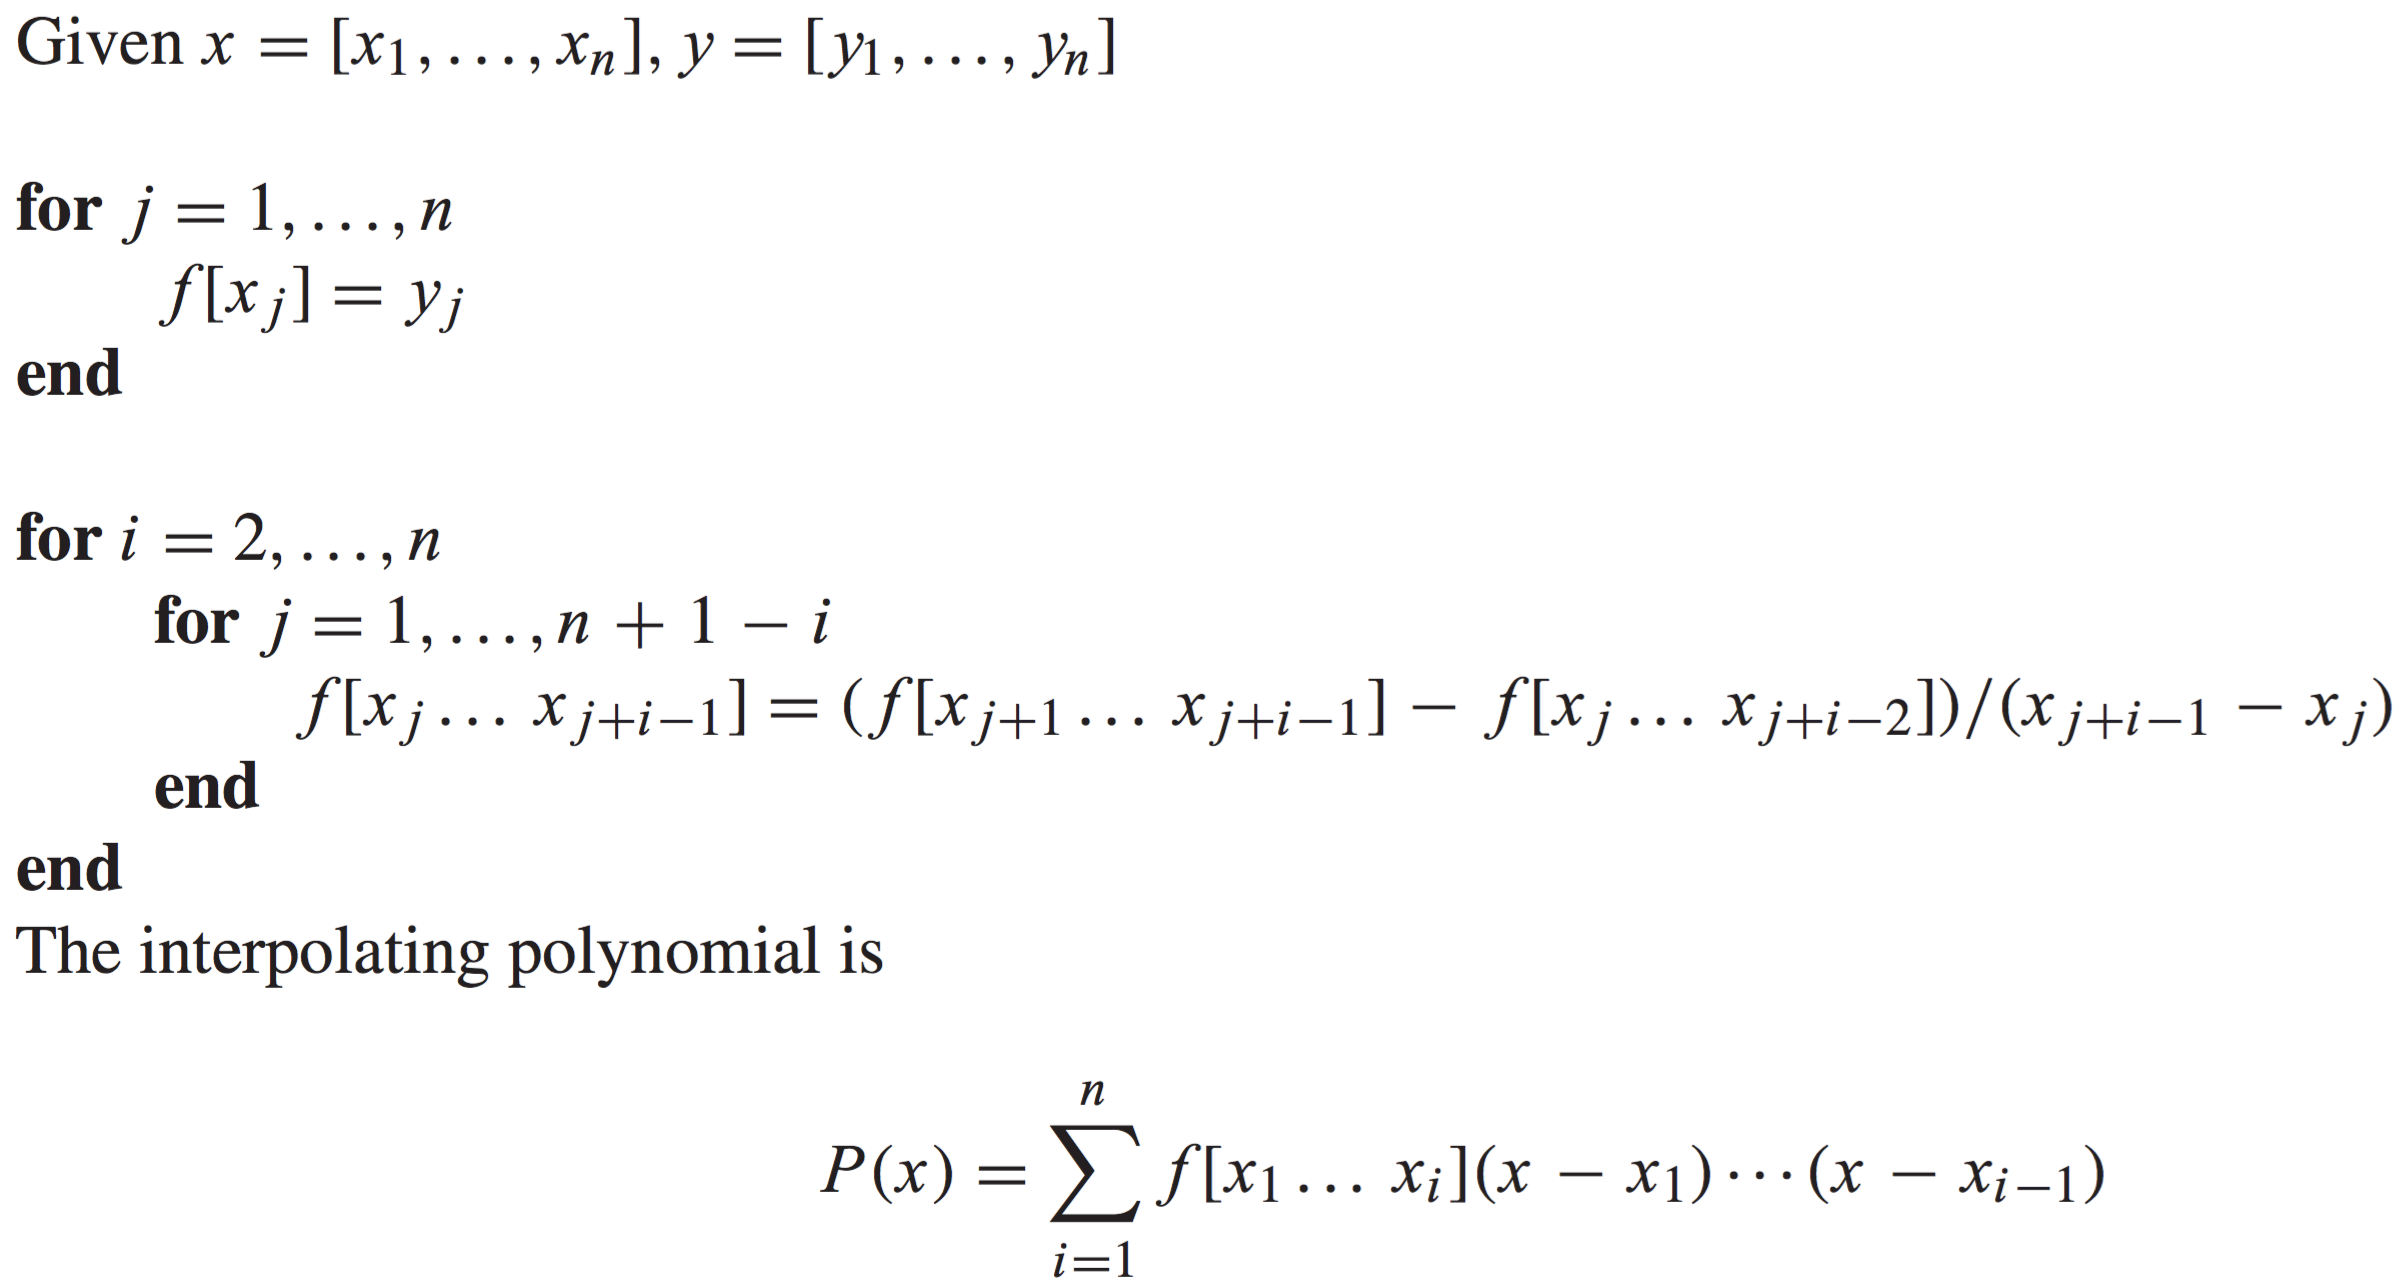
\includegraphics[scale=0.22]{newtondd_algorithm.png}
\end{center}

A recursive table in the form
\begin{center}
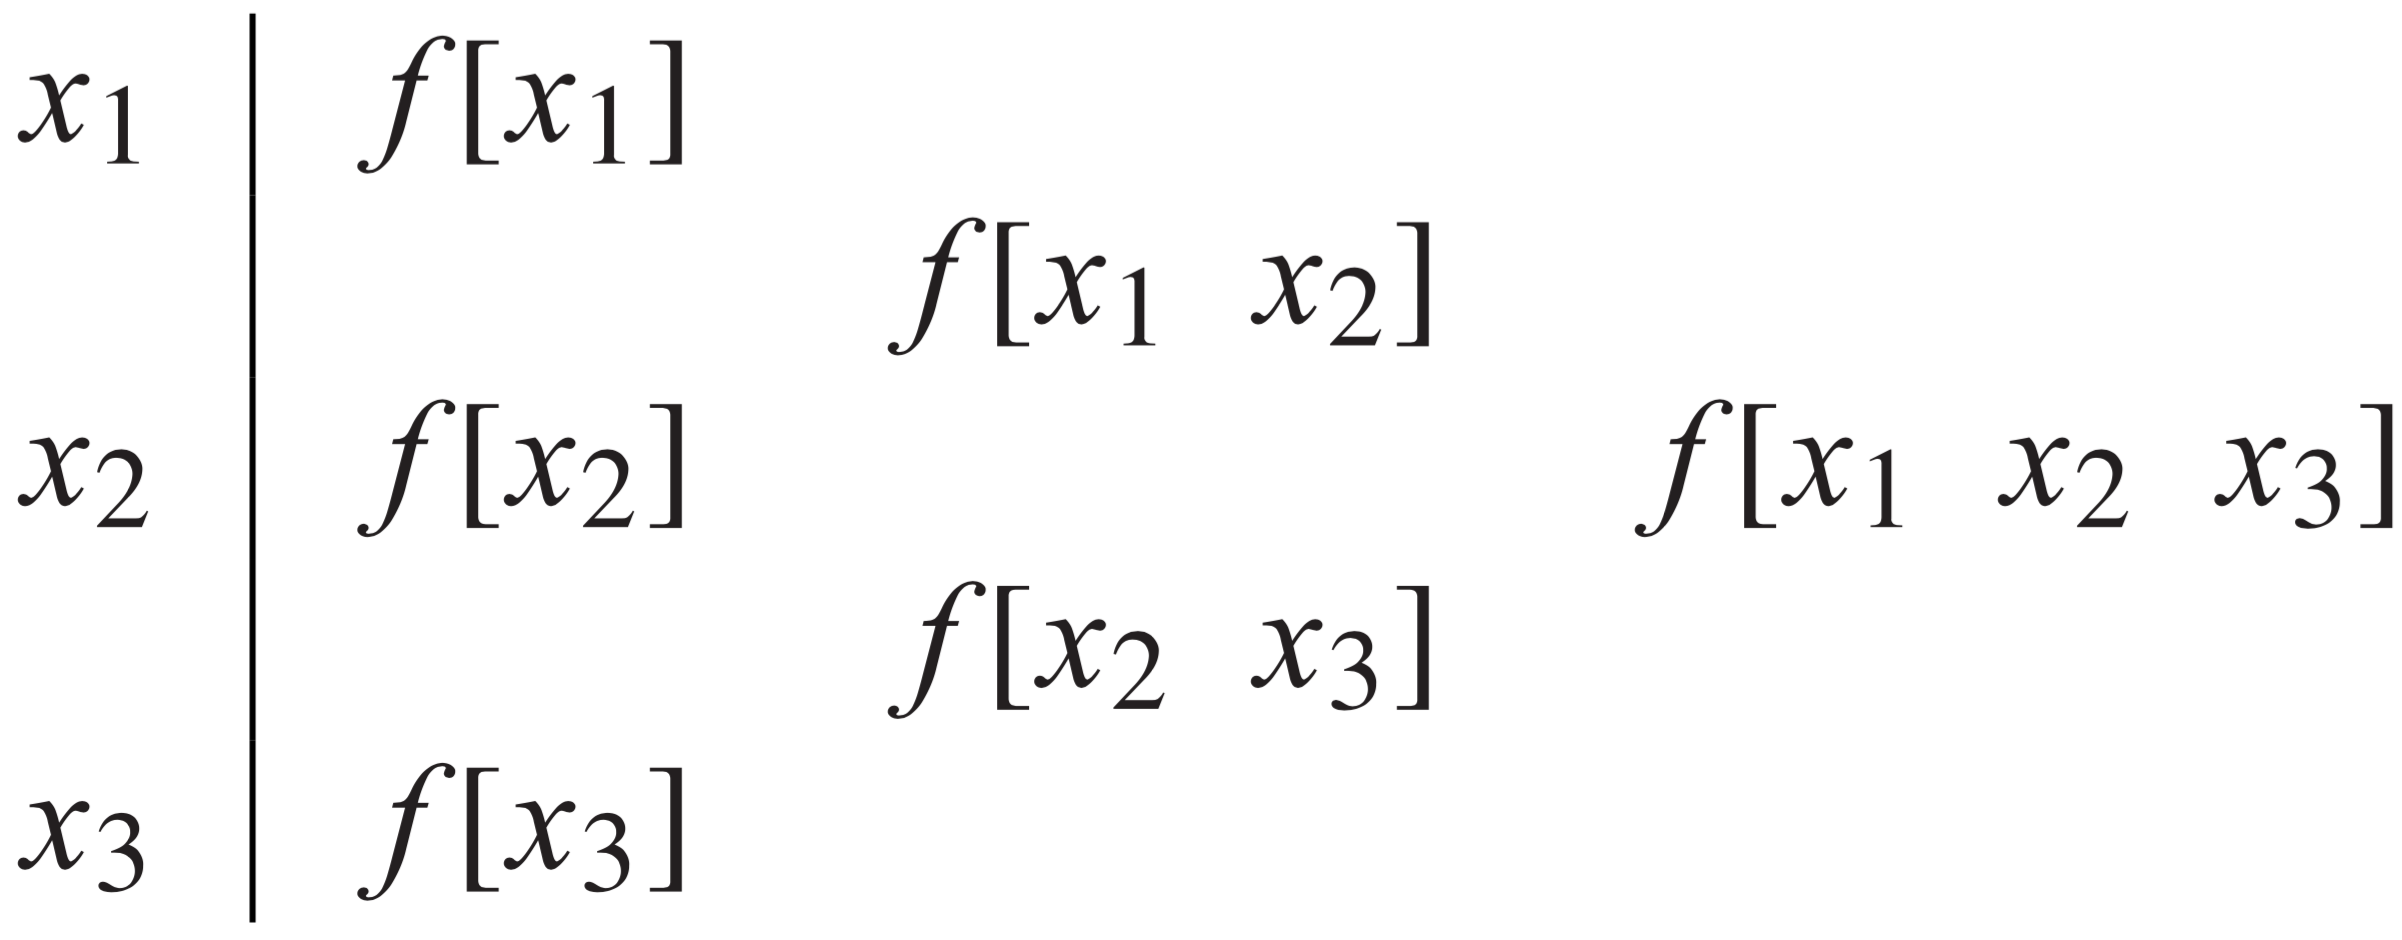
\includegraphics[scale=0.1]{newtondd.png}
\end{center}
can be made, and the top row gives the coefficients of the Newton's divided difference polynomial.

\subsection{Interpolation error}
%You should have an idea about where the interpolation error estimate comes from, but do not memorize the exact form.
\begin{theorem}
Assume that $P(x)$ is the (degree $n-1$ or less) interpolating polynomial fitting the $n$ points $(x_1,y_1),...,(x_n,y_n)$. The interpolation error is
$$
f(x)-P(x) = \frac{(x-x_1)(x-x_2)...(x-x_n)}{n!}f^{(n)}(c),
$$
where $c \in [\text{max}(x_1,...,x_n), \text{min}(x_1,...,x_n)]$.
\end{theorem}

\subsection{Runge's phenomenon}
Runge's phenomenon is the consequence of the magnitude of the derivatives of the interpolation function grows quickly when $n$ increases. This causes a "wiggle" effect at the ends of the interval and is solved by redistributing the interpolation nodes towards the ends. Speaking of which...

\subsection{Chebyshev Interpolation Nodes}
\begin{theorem}
On the interval $[a,b]$,
$$
x_i = \frac{b+a}{2} + \frac{b-a}{2}\cos{\frac{(2i-1)\pi}{2n}}
$$
for $i = 1, ..., n$. The inequality
$$
|(x-x_1)...(x-x_n)| \leq \frac{(\frac{b-a}{2})^n}{2^{n-1}}
$$
holds on $[a,b]$. The use of these nodes will minimize the interpolation error.
\end{theorem}